% questions.tex —— 2020 年·全国Ⅱ卷·文科 · 题目内容片段（无答案）
% 由 tools/generate_projects.py 依来源总账自 2020/2020_数学真题_全国2文_试题.md 生成，勿手改（改源 MD 后重跑）


\begin{gknotice}
\textbf{来源说明}：本题面依据固定源 PDF 的两页 A3 题面逐题转录，原卷印刷页码为 1123、1124。第 1123 面为选择题 1—12、填空题 13—16 与解答题 17、18；第 1124 面为解答题 19—23。全卷三处节头依次为「一、选择题」「二、填空题」「三、解答题」，题号与索引一致；所有数值、分式、根号与上下标均回原页 300—600 dpi 核对。

\textbf{解析归属}：固定源不附答案或解析；配套答案与解析均由本库按本题面独立复算（等级 D，非官方）。

\textbf{选做说明}：原卷第 22、23 题按选修模块二选一命制，题面未另加模块标题。本库全部收录，并以【A】标记第 22 题（选修 4—4 坐标系与参数方程）、【B】标记第 23 题（选修 4—5 不等式选讲），便于检索。

\textbf{图形说明}：第 3 题的钢琴键盘示意图、第 7 题的程序框图、第 20 题的三棱柱由项目内 TikZ 矢量源重绘；其余各题原页无图。
\end{gknotice}

\gkpart{一、选择题}

\begin{question}
\gkti{1}已知集合 $A=\{x\mid |x|<3,\ x\in\mathbf Z\}$，$B=\{x\mid |x|>1,\ x\in\mathbf Z\}$，则 $A\cap B=$\mbox{（　　）}

（A）$\varnothing$；（B）$\{-3,-2,2,3\}$；（C）$\{-2,0,2\}$；（D）$\{-2,2\}$。

\end{question}
\begin{question}
\gkti{2}$(1-\mathrm i)^4=$\mbox{（　　）}

（A）$-4$；（B）$4$；（C）$-4\mathrm i$；（D）$4\mathrm i$。

\Needspace{0.4\textheight}
\end{question}
\begin{question}
\gkti{3}如图，将钢琴上的 $12$ 个键依次记为 $a_1,a_2,\cdots,a_{12}$。设 $1\leqslant i<j<k\leqslant12$。若 $k-j=3$ 且 $j-i=4$，则称 $a_i,a_j,a_k$ 为原位大三和弦；若 $k-j=4$ 且 $j-i=3$，则称 $a_i,a_j,a_k$ 为原位小三和弦。用这 $12$ 个键可以构成的原位大三和弦与原位小三和弦的个数之和为\mbox{（　　）}

（A）$5$；（B）$8$；（C）$10$；（D）$15$。
\nopagebreak[4]
\begin{center}% 2020 全国Ⅱ卷 文3：钢琴键盘局部示意图（12 个键 a1—a12）
% 来源 PDF：普通高考/2020/2020全国2文(…).pdf 第 1 页（A3 横排），印面 1123，第 3 题题干下方
% 结构：七个白键 a1、a3、a5、a6、a8、a10、a12 自左至右排列；
%       五个黑键 a2、a4、a7、a9、a11 分别骑在相邻两白键的分界处，短于白键并从顶端下垂；
%       a5 与 a6 之间（第 3、4 个白键之间）没有黑键，对应键盘上 E—F 的半音间隙。
% 尺寸比：黑键宽 = 白键宽 × 2/3，黑键高 = 白键高 × 0.563（按原页 300 dpi 量取）。
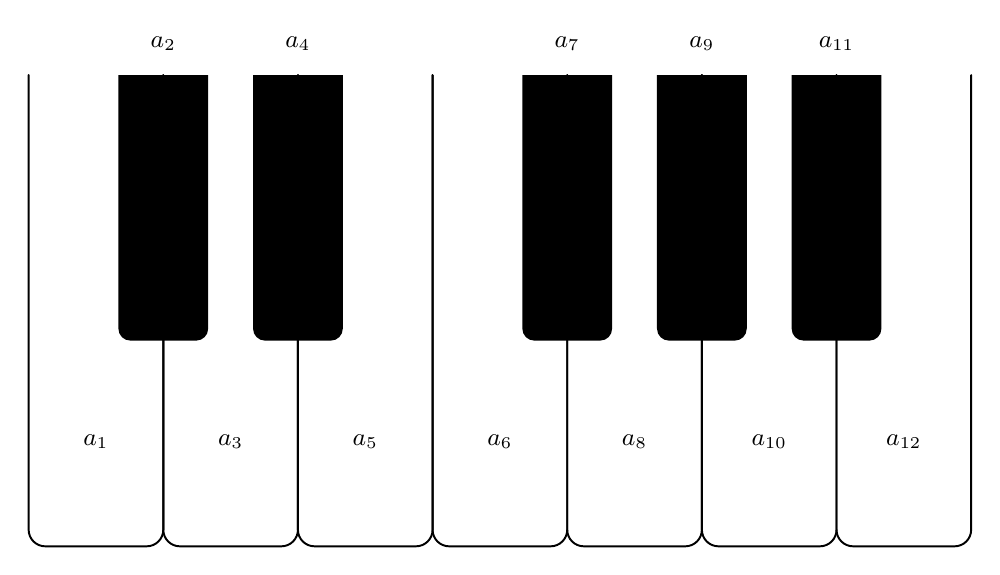
\begin{tikzpicture}[line width=0.7pt, font=\small,
  x=0.95cm, y=0.95cm, line cap=round, line join=round]
  \def\kw{1.8}    % 白键宽
  \def\kh{6.3}    % 白键高
  \def\bw{1.2}    % 黑键宽
  \def\bh{3.55}   % 黑键高

  % 白键：只画两侧竖线与圆角下沿，顶端不封口
  \foreach \i/\lab in {0/a_1, 1/a_3, 2/a_5, 3/a_6, 4/a_8, 5/a_{10}, 6/a_{12}} {
    \draw[rounded corners=6pt]
      ({\i*\kw},0) -- ({\i*\kw},-\kh) -- ({\i*\kw+\kw},-\kh) -- ({\i*\kw+\kw},0);
    \node at ({\i*\kw+\kw/2},-4.9) {$\lab$};
  }

  % 黑键：骑在白键分界处，实心，顶端齐平、下沿圆角
  \def\br{0.16}   % 黑键下沿圆角半径
  \foreach \b/\lab in {1.8/a_2, 3.6/a_4, 7.2/a_7, 9.0/a_9, 10.8/a_{11}} {
    \fill ({\b-\bw/2},0)
      -- ({\b-\bw/2},{-\bh+\br})
      arc[start angle=180, end angle=270, radius=\br]
      -- ({\b+\bw/2-\br},{-\bh})
      arc[start angle=270, end angle=360, radius=\br]
      -- ({\b+\bw/2},0) -- cycle;
    \node at ({\b},0.42) {$\lab$};
  }
\end{tikzpicture}
\end{center}
\nopagebreak[4]
\end{question}
\begin{question}
\gkti{4}在新冠肺炎疫情防控期间，某超市开通网上销售业务，每天能完成 $1200$ 份订单的配货，由于订单量大幅增加，导致订单积压。为解决困难，许多志愿者踊跃报名参加配货工作。已知该超市某日积压 $500$ 份订单未配货，预计第二天的新订单超过 $1600$ 份的概率为 $0.05$。志愿者每人每天能完成 $50$ 份订单的配货，为使第二天完成积压订单及当日订单的配货的概率不小于 $0.95$，则至少需要志愿者\mbox{（　　）}

（A）$10$ 名；（B）$18$ 名；（C）$24$ 名；（D）$32$ 名。

\end{question}
\begin{question}
\gkti{5}已知单位向量 $\boldsymbol a$，$\boldsymbol b$ 的夹角为 $60^\circ$，则在下列向量中，与 $\boldsymbol b$ 垂直的是\mbox{（　　）}

（A）$\boldsymbol a+2\boldsymbol b$；（B）$2\boldsymbol a+\boldsymbol b$；（C）$\boldsymbol a-2\boldsymbol b$；（D）$2\boldsymbol a-\boldsymbol b$。

\end{question}
\begin{question}
\gkti{6}记 $S_n$ 为等比数列 $\{a_n\}$ 的前 $n$ 项和。若 $a_5-a_3=12$，$a_6-a_4=24$，则 $\dfrac{S_n}{a_n}=$\mbox{（　　）}

（A）$2^n-1$；（B）$2-2^{1-n}$；（C）$2-2^{n-1}$；（D）$2^{1-n}-1$。

\Needspace{0.4\textheight}
\end{question}
\begin{question}
\gkti{7}执行下面的程序框图，若输入的 $k=0$，$a=0$，则输出的 $k$ 为\mbox{（　　）}

（A）$2$；（B）$3$；（C）$4$；（D）$5$。
\nopagebreak[4]
\begin{center}% 2020 全国Ⅱ卷 文7：程序框图
% 来源 PDF：普通高考/2020/2020全国2文(…).pdf 第 1 页（A3 横排），印面 1123，第 7 题左侧
% 结构：开始 → 输入 k, a → [ a = 2a+1 → k = k+1 → 判断 a>10 ]，判断为「否」回到 a = 2a+1，
%       判断为「是」经输出 k 到结束；循环分支从判断框左顶点引出，向上折回处理框 a = 2a+1 上方。
% 形状约定：终端框为圆角矩形，输入/输出框为平行四边形，处理框为矩形，判断框为菱形。
\begin{tikzpicture}[line width=0.7pt, font=\small, >=Stealth,
  line cap=round, line join=round]

  % 终端框：开始 / 结束
  \node[draw, rounded corners=4pt, minimum width=1.5cm, minimum height=0.78cm,
        inner sep=2pt] (sta) at (0,0) {开始};
  \node[draw, rounded corners=4pt, minimum width=1.5cm, minimum height=0.78cm,
        inner sep=2pt] (fin) at (0,-11.0) {结束};

  % 输入框（平行四边形，上边相对下边右移）
  \draw (-1.40,-1.45) -- (2.40,-1.45) -- (1.40,-2.25) -- (-2.40,-2.25) -- cycle;
  \node at (0,-1.85) {输入 $k$，$a$};

  % 输出框（同形）
  \draw (-1.40,-8.95) -- (2.40,-8.95) -- (1.40,-9.75) -- (-2.40,-9.75) -- cycle;
  \node at (0,-9.35) {输出 $k$};

  % 处理框
  \node[draw, minimum width=3.4cm, minimum height=0.78cm, inner sep=2pt]
        (p1) at (0,-3.70) {$a=2a+1$};
  \node[draw, minimum width=3.1cm, minimum height=0.78cm, inner sep=2pt]
        (p2) at (0,-5.45) {$k=k+1$};

  % 判断框
  \node[draw, diamond, aspect=4.2, minimum width=4.8cm, inner sep=1pt]
        (jud) at (0,-7.40) {$a>10$};

  % 主干流程
  \draw[->] (sta.south) -- (0,-1.45);
  \draw[->] (0,-2.25) -- (p1.north);
  \draw[->] (p1.south) -- (p2.north);
  \draw[->] (p2.south) -- (jud.north);
  \draw[->] (jud.south) -- (0,-8.95);
  \draw[->] (0,-9.75) -- (fin.north);

  % 循环分支：判断框左顶点 → 左 → 上 → 折回处理框上方，箭头指向主干
  \draw[->] (jud.west) -- (-3.45,-7.40) -- (-3.45,-3.00) -- (-0.05,-3.00);

  % 分支标注
  \node at (-2.80,-7.02) {否};
  \node at (0.45,-8.30) {是};
\end{tikzpicture}
\end{center}
\nopagebreak[4]
\end{question}
\begin{question}
\gkti{8}若过点 $(2,1)$ 的圆与两坐标轴都相切，则圆心到直线 $2x-y-3=0$ 的距离为\mbox{（　　）}

（A）$\dfrac{\sqrt5}5$；（B）$\dfrac{2\sqrt5}5$；（C）$\dfrac{3\sqrt5}5$；（D）$\dfrac{4\sqrt5}5$。

\end{question}
\begin{question}
\gkti{9}设 $O$ 为坐标原点，直线 $x=a$ 与双曲线 $C:\dfrac{x^2}{a^2}-\dfrac{y^2}{b^2}=1$（$a>0$，$b>0$）的两条渐近线分别交于 $D$，$E$ 两点。若 $\triangle ODE$ 的面积为 $8$，则 $C$ 的焦距的最小值为\mbox{（　　）}

（A）$4$；（B）$8$；（C）$16$；（D）$32$。

\end{question}
\begin{question}
\gkti{10}设函数 $f(x)=x^3-\dfrac1{x^3}$，则 $f(x)$\mbox{（　　）}

（A）是奇函数，且在 $(0,+\infty)$ 单调递增；（B）是奇函数，且在 $(0,+\infty)$ 单调递减；（C）是偶函数，且在 $(0,+\infty)$ 单调递增；（D）是偶函数，且在 $(0,+\infty)$ 单调递减。

\end{question}
\begin{question}
\gkti{11}已知 $\triangle ABC$ 是面积为 $\dfrac{9\sqrt3}4$ 的等边三角形，且其顶点都在球 $O$ 的球面上。若球 $O$ 的表面积为 $16\pi$，则 $O$ 到平面 $ABC$ 的距离为\mbox{（　　）}

（A）$\sqrt3$；（B）$\dfrac32$；（C）$1$；（D）$\dfrac{\sqrt3}2$。

\end{question}
\begin{question}
\gkti{12}若 $2^x-2^y<3^{-x}-3^{-y}$，则\mbox{（　　）}

（A）$\ln(y-x+1)>0$；（B）$\ln(y-x+1)<0$；（C）$\ln|x-y|>0$；（D）$\ln|x-y|<0$。

\end{question}
\gkpart{二、填空题}

\begin{question}
\gkti{13}若 $\sin x=-\dfrac23$，则 $\cos2x=$\gkblank{}。

\end{question}
\begin{question}
\gkti{14}记 $S_n$ 为等差数列 $\{a_n\}$ 的前 $n$ 项和。若 $a_1=-2$，$a_2+a_6=2$，则 $S_{10}=$\gkblank{}。

\end{question}
\begin{question}
\gkti{15}若 $x$，$y$ 满足约束条件 $\begin{cases}x+y\geqslant-1,\\x-y\geqslant-1,\\2x-y\leqslant1,\end{cases}$ 则 $z=x+2y$ 的最大值是\gkblank{}。

\end{question}
\begin{question}
\gkti{16}设有下列四个命题：

$p_1$：两两相交且不过同一点的三条直线必在同一平面内；

$p_2$：过空间中任意三点有且仅有一个平面；

$p_3$：若空间两条直线不相交，则这两条直线平行；

$p_4$：若直线 $l\subset$ 平面 $\alpha$，直线 $m\perp$ 平面 $\alpha$，则 $m\perp l$。

则下述命题中所有真命题的序号是\gkblank{}。

① $p_1\wedge p_4$；② $p_1\wedge p_2$；③ $\neg p_2\vee p_3$；④ $\neg p_3\vee\neg p_4$。

\end{question}
\gkpart{三、解答题}

\begin{question}
\gkti{17}$\triangle ABC$ 的内角 $A$，$B$，$C$ 的对边分别为 $a$，$b$，$c$，已知 $\cos^2\left(\dfrac\pi2+A\right)+\cos A=\dfrac54$。

（1） 求 $A$；

（2） 若 $b-c=\dfrac{\sqrt3}3a$，证明：$\triangle ABC$ 是直角三角形。

\end{question}
\begin{question}
\gkti{18}某沙漠地区经过治理，生态系统得到很大改善，野生动物数量有所增加。为调查该地区某种野生动物的数量，将其分成面积相近的 $200$ 个地块，从这些地块中用简单随机抽样的方法抽取 $20$ 个作为样区，调查得到样本数据 $(x_i,y_i)$（$i=1,2,\cdots,20$），其中 $x_i$ 和 $y_i$ 分别表示第 $i$ 个样区的植物覆盖面积（单位：公顷）和这种野生动物的数量，并计算得

\nopagebreak[4]
\[\sum_{i=1}^{20}x_i=60,\qquad \sum_{i=1}^{20}y_i=1200,\]
\nopagebreak[4]
\[\sum_{i=1}^{20}(x_i-\bar x)^2=80,\qquad \sum_{i=1}^{20}(y_i-\bar y)^2=9000,\qquad \sum_{i=1}^{20}(x_i-\bar x)(y_i-\bar y)=800.\]

（1） 求该地区这种野生动物数量的估计值（这种野生动物数量的估计值等于样区这种野生动物数量的平均数乘以地块数）；

（2） 求样本 $(x_i,y_i)$（$i=1,2,\cdots,20$）的相关系数（精确到 $0.01$）；

（3） 根据现有统计资料，各地块间植物覆盖面积差异很大。为提高样本的代表性以获得该地区这种野生动物数量更准确的估计，请给出一种你认为更合理的抽样方法，并说明理由。

附：相关系数 $r=\dfrac{\sum\limits_{i=1}^n(x_i-\bar x)(y_i-\bar y)}{\sqrt{\sum\limits_{i=1}^n(x_i-\bar x)^2\sum\limits_{i=1}^n(y_i-\bar y)^2}}$，$\sqrt2\approx1.414$。

\end{question}
\begin{question}
\gkti{19}已知椭圆 $C_1:\dfrac{x^2}{a^2}+\dfrac{y^2}{b^2}=1$（$a>b>0$）的右焦点 $F$ 与抛物线 $C_2$ 的焦点重合，$C_1$ 的中心与 $C_2$ 的顶点重合。过 $F$ 且与 $x$ 轴垂直的直线交 $C_1$ 于 $A$，$B$ 两点，交 $C_2$ 于 $C$，$D$ 两点，且 $|CD|=\dfrac43|AB|$。

（1） 求 $C_1$ 的离心率；

（2） 若 $C_1$ 的四个顶点到 $C_2$ 的准线距离之和为 $12$，求 $C_1$ 与 $C_2$ 的标准方程。

\Needspace{0.4\textheight}
\end{question}
\begin{question}
\gkti{20}如图，已知三棱柱 $ABC-A_1B_1C_1$ 的底面是正三角形，侧面 $BB_1C_1C$ 是矩形，$M$，$N$ 分别为 $BC$，$B_1C_1$ 的中点，$P$ 为 $AM$ 上一点。过 $B_1C_1$ 和 $P$ 的平面交 $AB$ 于 $E$，交 $AC$ 于 $F$。

（1） 证明：$AA_1\parallel MN$，且平面 $A_1AMN\perp$ 平面 $EB_1C_1F$；

（2） 设 $O$ 为 $\triangle A_1B_1C_1$ 的中心，若 $AO=AB=6$，$AO\parallel$ 平面 $EB_1C_1F$，且 $\angle MPN=\dfrac\pi3$，求四棱锥 $B-EB_1C_1F$ 的体积。
\nopagebreak[4]
\begin{center}% 2020 全国Ⅱ卷 文20：三棱柱 ABC-A1B1C1 与截面四边形 EB1C1F
% 来源 PDF：普通高考/2020/2020全国2文(…).pdf 第 2 页（A3 横排），印面 1124，第 20 题题干下方
% 结构：底面 ABC 为正三角形，侧面 BB1C1C 为矩形（BB1⊥BC）；M、N 为 BC、B1C1 的中点，
%       O 为 △A1B1C1 的中心，P 为 AM 上一点（AP = AM/3），截面 EB1C1F 与底面交于 EF（EF∥BC）。
% 实线：A1A、A1B1、A1C1、B1C1、C1C、CB、BA、B1B、NM、B1E，以及原页所绘的矩形对角线 BC1；
% 虚线：AC、AO、AM（含点 P）、EF、FC1、PN（原页为标出 ∠MPN 而作）。
% 投影取自原页 300 dpi 量取的顶点位置，M、N、O 按中点/重心精确算出，E、F、P 取 AM 的三等分点。
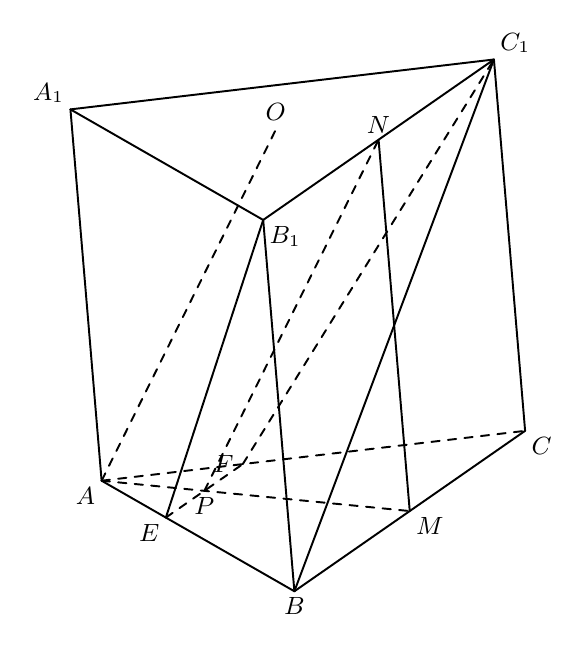
\begin{tikzpicture}[line width=0.7pt, font=\small,
  x=0.72cm, y=0.72cm, line cap=round, line join=round]

  % 顶点
  \coordinate (A1) at (0.15,9.50);
  \coordinate (B1) at (3.55,7.55);
  \coordinate (C1) at (7.62,10.38);
  \coordinate (A)  at (0.70,2.95);
  \coordinate (B)  at (4.10,1.00);
  \coordinate (C)  at (8.17,3.83);

  % 中点、重心与截面点
  \coordinate (M)  at (6.135,2.415);
  \coordinate (N)  at (5.585,8.965);
  \coordinate (O)  at (3.773,9.143);
  \coordinate (E)  at (1.833,2.300);
  \coordinate (F)  at (3.190,3.243);
  \coordinate (P)  at (2.512,2.772);

  % 可见棱
  \draw (A1) -- (A);
  \draw (A1) -- (B1);
  \draw (A1) -- (C1);
  \draw (B1) -- (C1);
  \draw (B1) -- (B);
  \draw (C1) -- (C);
  \draw (B)  -- (C);
  \draw (A)  -- (B);

  % 中位线与截面可见边
  \draw (N) -- (M);
  \draw (B1) -- (E);

  % 矩形 BB1C1C 的对角线 BC1（原页实线）
  \draw (B) -- (C1);

  % 被遮挡的棱与内部辅助线
  \draw[dashed] (A) -- (C);
  \draw[dashed] (A) -- (O);
  \draw[dashed] (A) -- (M);
  \draw[dashed] (E) -- (F);
  \draw[dashed] (F) -- (C1);
  \draw[dashed] (P) -- (N);

  % 顶点标注
  \node[above left,  inner sep=2pt] at (A1) {$A_1$};
  \node[below left,  inner sep=2pt] at (A)  {$A$};
  \node[below,       inner sep=2pt] at (B)  {$B$};
  \node[below right, inner sep=2pt] at (C)  {$C$};
  \node[above right, inner sep=2pt] at (C1) {$C_1$};
  \node[below right, inner sep=2pt] at (B1) {$B_1$};
  \node[above,       inner sep=2pt] at (N)  {$N$};
  \node[above,       inner sep=3pt] at (O)  {$O$};
  \node[below right, inner sep=2pt] at (M)  {$M$};
  \node[below left,  inner sep=2pt] at (E)  {$E$};
  \node[left,        inner sep=3pt] at (F)  {$F$};
  \node[below,       inner sep=2pt] at (P)  {$P$};
\end{tikzpicture}
\end{center}
\nopagebreak[4]
\end{question}
\begin{question}
\gkti{21}已知函数 $f(x)=2\ln x+1$。

（1） 若 $f(x)\leqslant2x+c$，求 $c$ 的取值范围；

（2） 设 $a>0$ 时，讨论函数 $g(x)=\dfrac{f(x)-f(a)}{x-a}$ 的单调性。

\end{question}
\begin{question}
\gkti{22}\textbf{【A】（选修 4—4：坐标系与参数方程）} 已知曲线 $C_1$，$C_2$ 的参数方程分别为 $C_1:\begin{cases}x=4\cos^2\theta,\\y=4\sin^2\theta\end{cases}$（$\theta$ 为参数），$C_2:\begin{cases}x=t+\dfrac1t,\\y=t-\dfrac1t\end{cases}$（$t$ 为参数）。

（1） 将 $C_1$，$C_2$ 的参数方程化为普通方程；

（2） 以坐标原点为极点，$x$ 轴正半轴为极轴建立极坐标系。设 $C_1$，$C_2$ 的交点为 $P$，求圆心在极轴上，且经过极点和 $P$ 的圆的极坐标方程。

\end{question}
\begin{question}
\gkti{23}\textbf{【B】（选修 4—5：不等式选讲）} 已知函数 $f(x)=|x-a^2|+|x-2a+1|$。

（1） 当 $a=2$ 时，求不等式 $f(x)\geqslant4$ 的解集；

（2） 若 $f(x)\geqslant4$，求 $a$ 的取值范围。

\end{question}